%-------------------------------------------------------------------------------
%-------------------------------------------------------------------------------
\begin{frame}
Human capital is defined as:
\vspace{\baselineskip}

\begin{quote}
The knowledge, skills, competencies and attributes embodied in individuals that facilitate
the creation of personal, social and economic well-being.
\end{quote}\vspace{-0.5pt} \hspace{6cm} - OECD (2001)
\end{frame}

%-------------------------------------------------------------------------------
%-------------------------------------------------------------------------------
\begin{frame}
	\begin{figure}
		\caption{Foundational work}
		\centering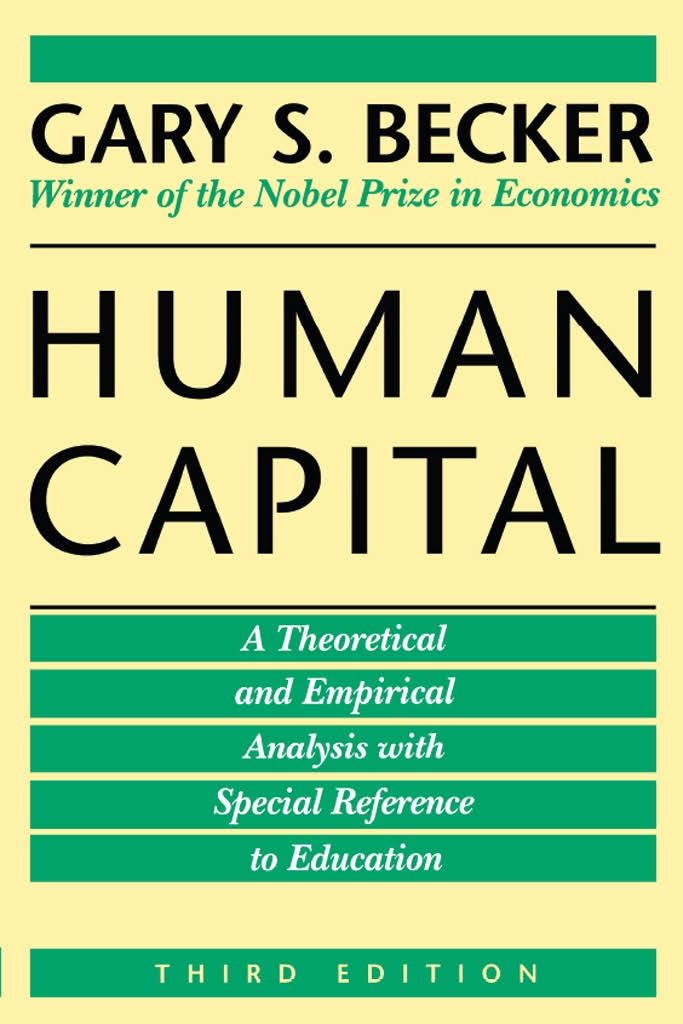
\includegraphics[width=0.40\linewidth]{fig-human-capital-treatise}
	\end{figure}
\end{frame}


%-------------------------------------------------------------------------------
%-------------------------------------------------------------------------------
\begin{frame}
\centering
\begin{threeparttable}\footnotesize
  \caption{Lecture plan}
  \begin{tabular}{ll}\toprule
  Date & Topic \\\midrule
05/09/18 & Introduction to the economics of human capital\\
05/30/18 & Returns to schooling \\
06/06/18 & Multidimensionality of skills \\
06/13/18 & Static model of educational choice \\
06/20/18 & Dynamic model of human capital accumulation \\
06/27/18 & Intergenerational transmission of human capital\\
\bottomrule
\end{tabular}
\end{threeparttable}
\end{frame}
%-------------------------------------------------------------------------------
%-------------------------------------------------------------------------------
\begin{frame}\textbf{Open Source Economics}\vspace{0.3cm}

\begin{itemize}\setlength\itemsep{1em}
\item \textbf{respy}, Python package for the simulation and estimation of a prototypical finite-horizon dynamic discrete choice model
\item \textbf{grmpy}, Python package for the simulation and estimation of generalized Roy model
\end{itemize}
\end{frame}
%-------------------------------------------------------------------------------
%-------------------------------------------------------------------------------
\begin{frame}
	\begin{figure}
		\caption{Guest lecture by Benedikt Kauf}
		\centering\scalebox{0.15}{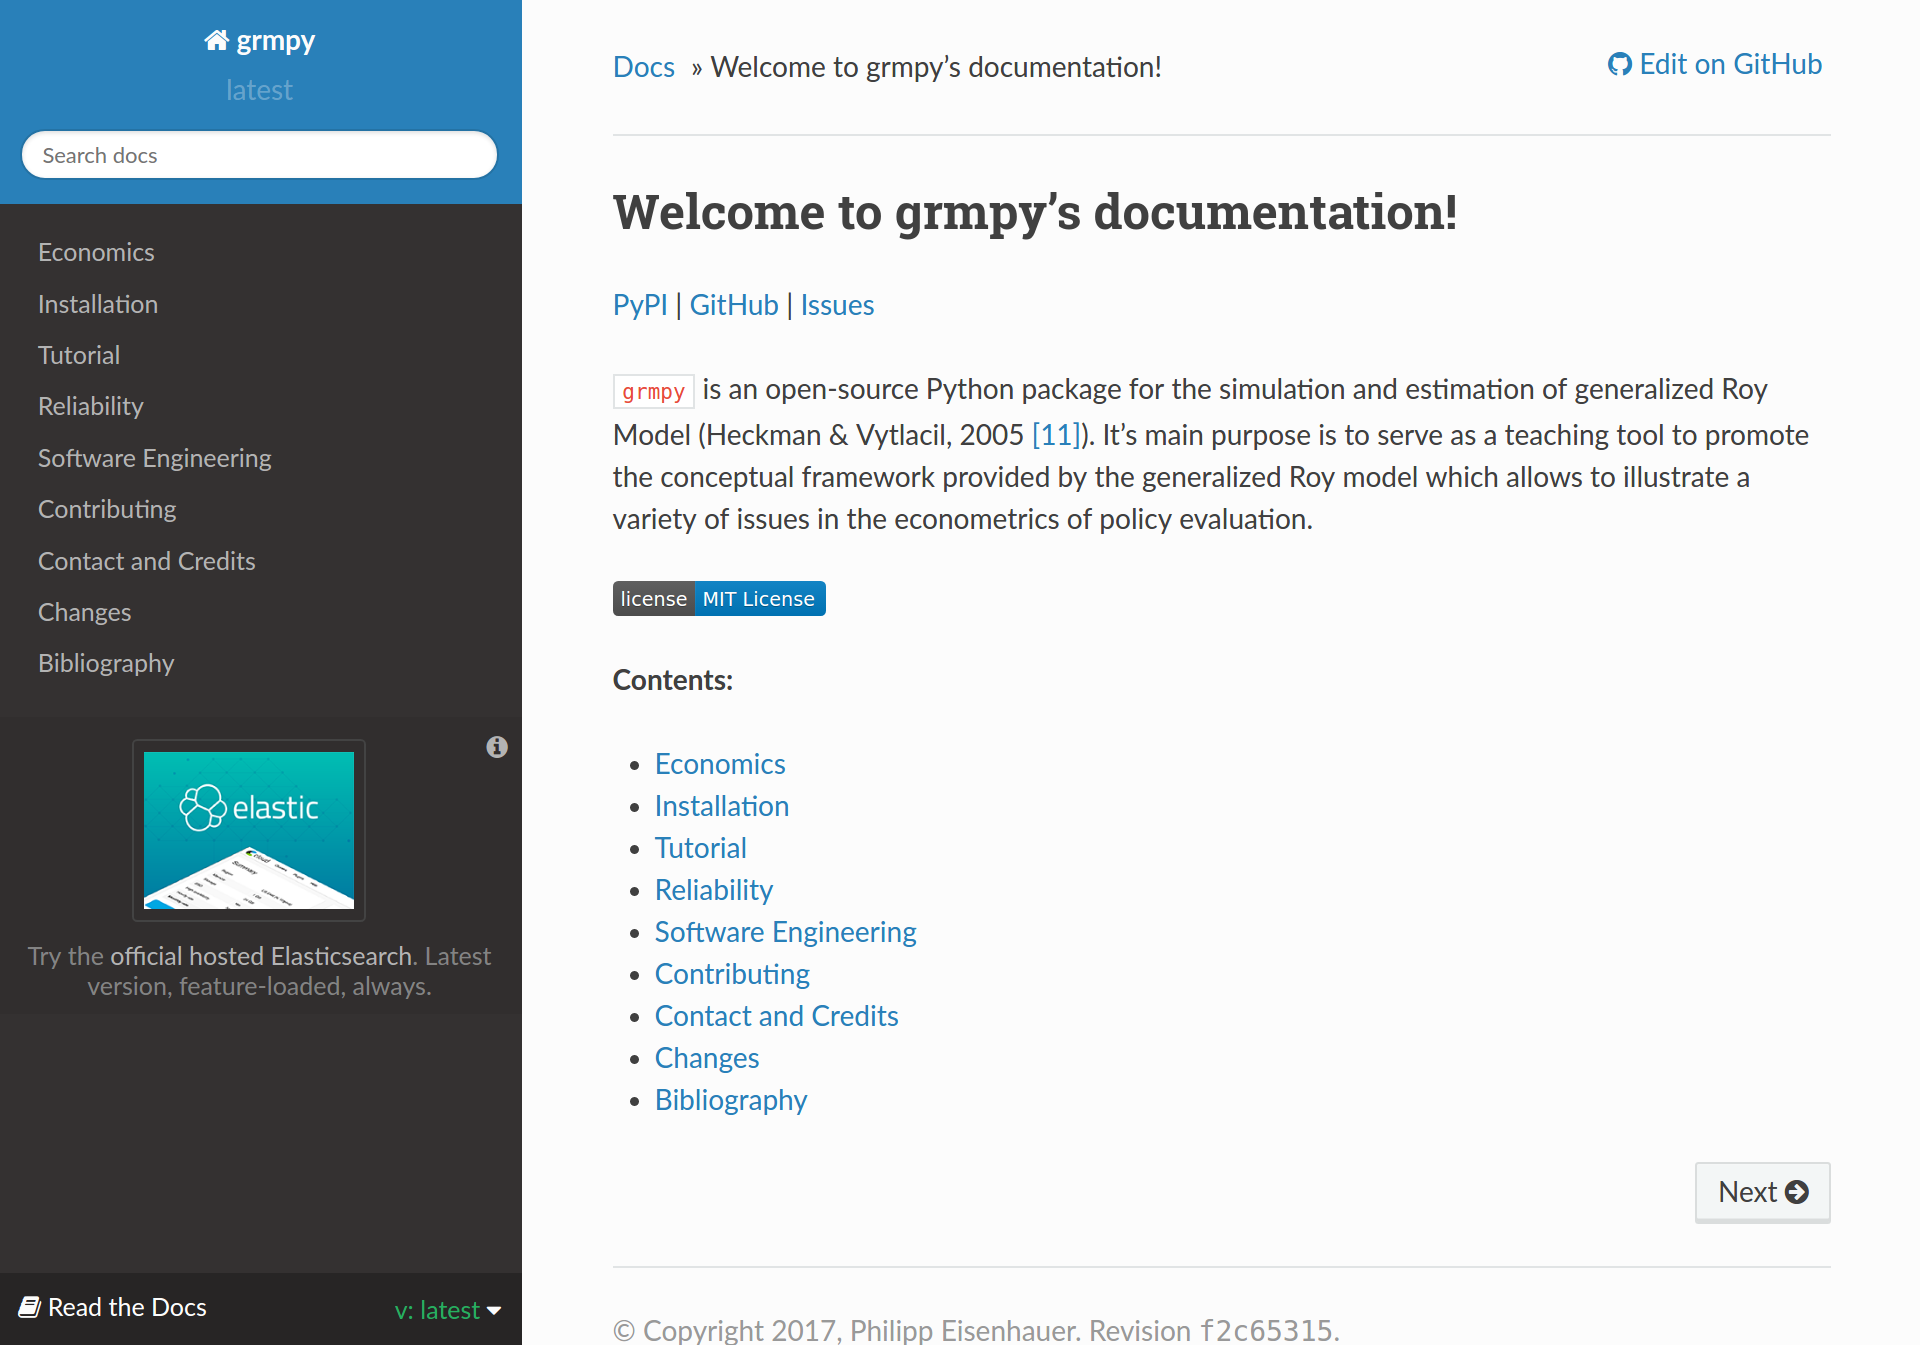
\includegraphics{fig-documentation-grmpy}}
	\end{figure}
\end{frame}
%-------------------------------------------------------------------------------
%-------------------------------------------------------------------------------
\begin{frame}
	\begin{figure}
		\caption{Guest lecture by Janos Gabler}
		\centering\scalebox{0.15}{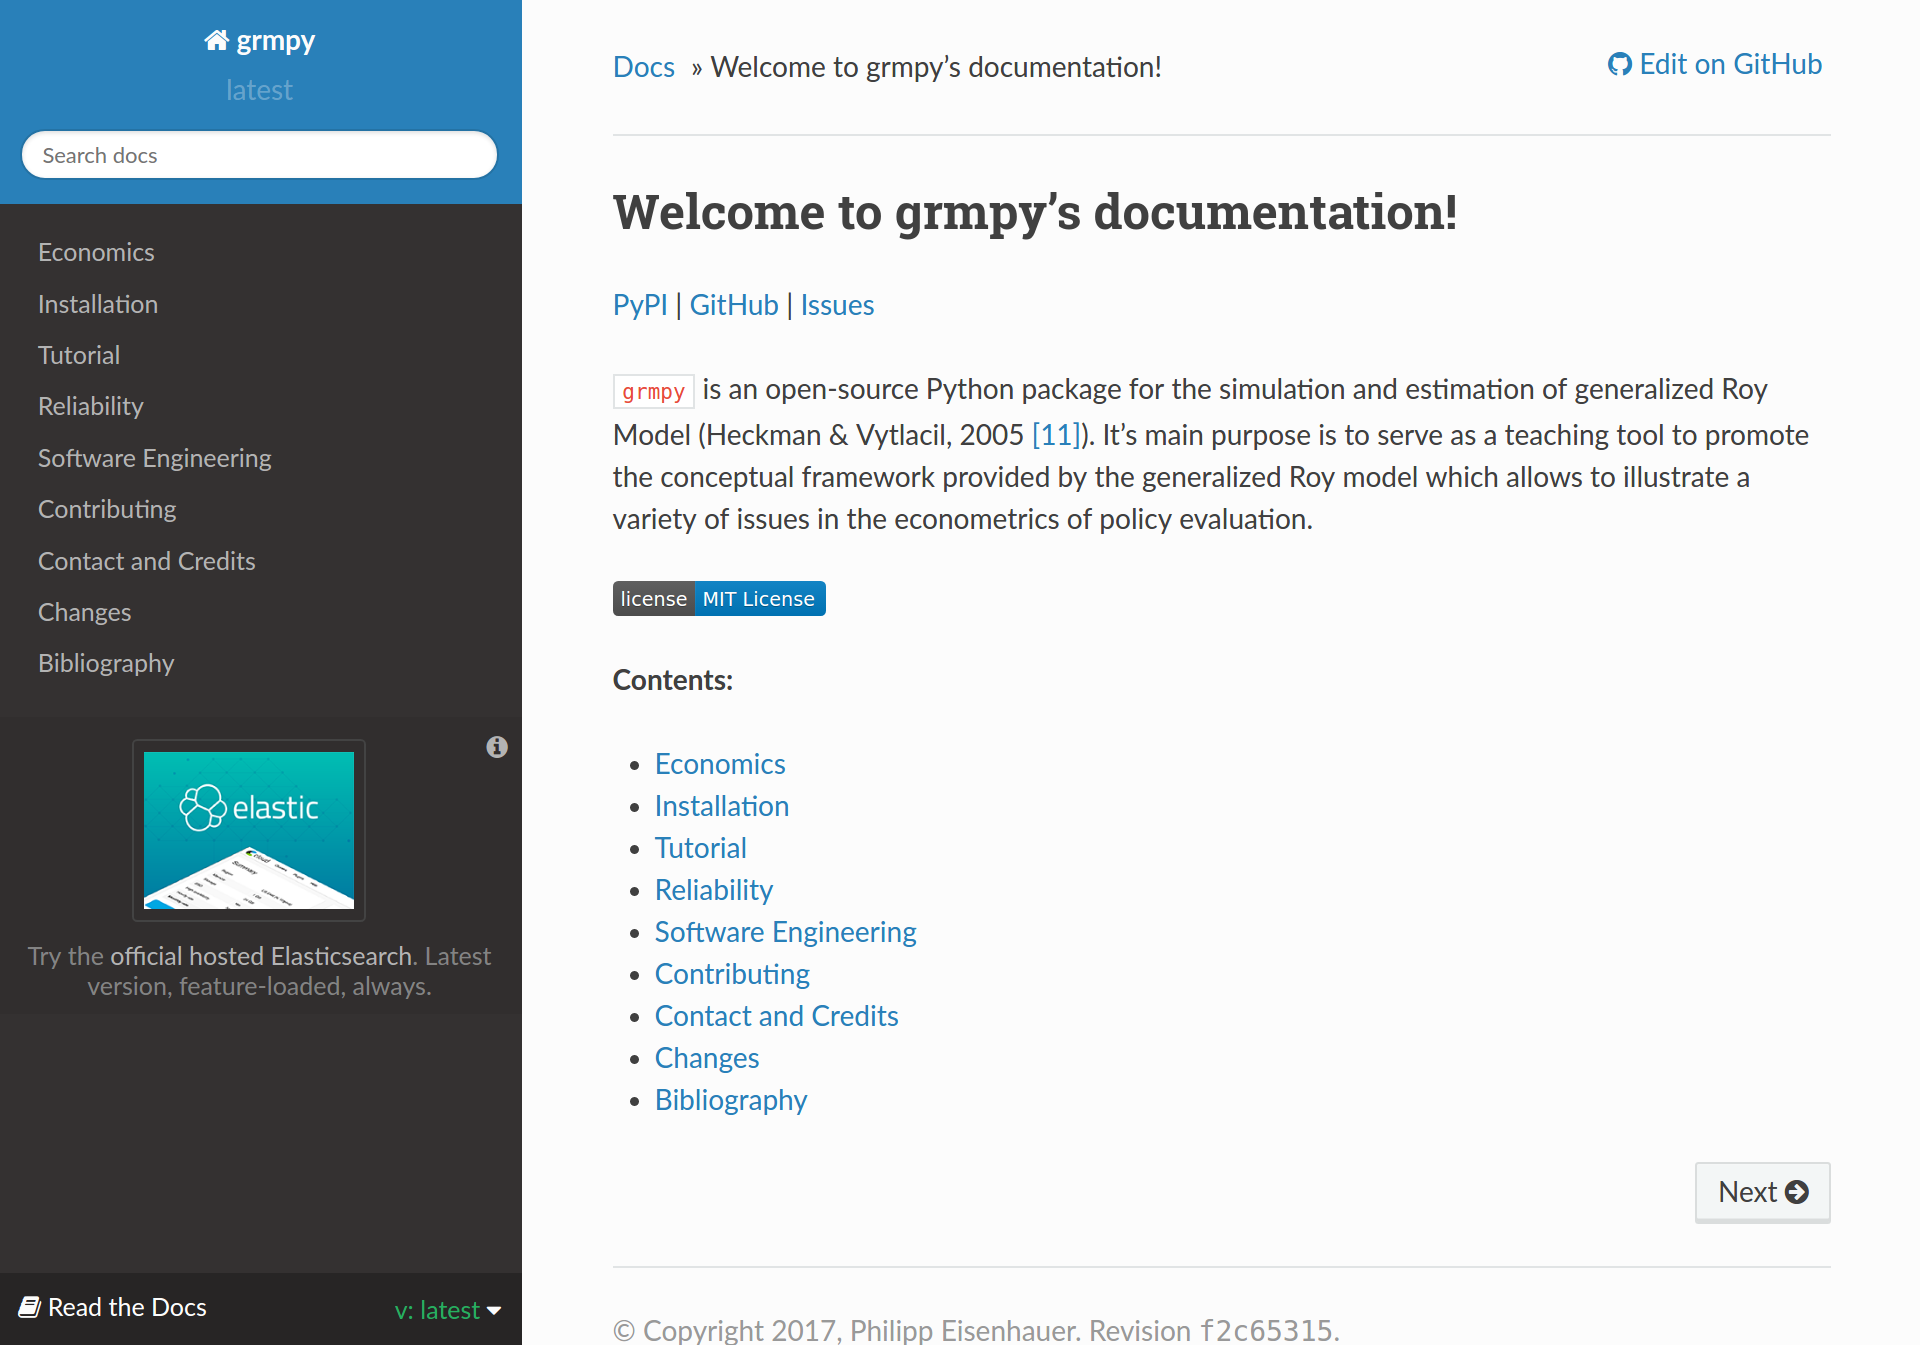
\includegraphics[width=1920px, height=1345px]{fig-documentation-respy}}
	\end{figure}
\end{frame}
%-------------------------------------------------------------------------------
%-------------------------------------------------------------------------------
\begin{frame}
	\textbf{Course Website}\vspace{0.3cm}

You find all information about the course on our website.

\begin{center}
\url{https://github.com/HumanCapitalEconomics/course/}
\end{center}

This includes the lecture dates, topics, reading list, and the slides.\vspace{0.3cm}

If you have further questions, please feel free to contact us using

\includegraphics[scale=0.5]{fig-gitter}.

\end{frame}
%-------------------------------------------------------------------------------
%-------------------------------------------------------------------------------
\begin{frame}
	\textbf{Related Courses}\vspace{0.3cm}

We offer several other courses on the material presented here.

	\begin{center}
	\url{https://github.com/policyMetrics}
	\end{center}


	\begin{itemize}\setlength\itemsep{1em}
	\item Econometrics of policy evaluation
	\item The nature of human motivation, skill formation, and labor market outcomes
	\end{itemize}

\end{frame}
%-------------------------------------------------------------------------------
%-------------------------------------------------------------------------------
\begin{frame}
	\textbf{Related Issues}\vspace{0.3cm}

	\begin{itemize}\setlength\itemsep{1em}
	\item Thesis Projects
	\item Reference Letters
	\end{itemize}
\end{frame}
